\documentclass[a4paper,12pt,russian]{extarticle}
\usepackage{../MyPackages/commands}
\RequirePackage{caption}
\usepackage{graphicx}
\newcommand{\Pn}[3]{P^{(#1)} \br{#2,#3}}
\newcommand{\G}{\Gamma}
\newcommand{\e}{\eta_i^{(1)}}
\newcommand{\ee}{\eta_i^{(2)}}
\renewcommand{\b}{b^{(1)}}
\newcommand{\bb}{b^{(2)}}
\newcommand{\iakt}{[\tau_{i},\tau_{i+1})}
\newcommand{\Gr}[1]{\Gamma^{(#1)}}
\newcommand{\Mark}{\{(\G_i, \vk_i); i \geqslant 0\}}
%\newcommand{\Markk}[0]{\brrr{ \vk_i, i \geqslant 0}}
%\newcommand{\Markkhat}[0]{\brrr{ \hat{\vk}_i, i \geqslant 1}}
%\newcommand{\Markkhata}[0]{\brrr{ \hat{\vk}_i\br{a}, i \geqslant 1}}
%\newcommand{\Markkhato}[0]{\brrr{ \hat{\vk}_i\br{0}, i \geqslant 1}}
%\newcommand{\Markkhatoa}[0]{\brrr{ \hat{\hat{\vk}}_i\br{a}, i \geqslant 1}}
\usepackage[Magistr]{../MyPackages/ptvstyle}
%\selectlanguage{russian}
\title{Моделирование и анализ системы обслуживания конфликтных потоков в классе приоритетных алгоритмов}
\author{студент группы 85М1\\ Кочеганов В.~М.}
\advisor{к.ф.-м.н., доцент \\ Зорин А.~В.}
\chief{д.ф.-м.н., профессор \\ Федоткин М.~А.}
\date{2014}
\newcommand{\p}{\hat{p}}
\newcommand{\gam}[2]{\Gamma^{\left( #1 , #2 \right)} }
\newcommand{\T}[2]{T^{\left( #1 , #2 \right)} }
\newcommand{\ga}[1]{\Gamma^{\left( #1 \right)} }
\newcommand{\Tt}[1]{T^{\left( #1 \right)} }
%\newcommand*{\hm}[1]{#1\nobreak\discretionary{}%
%{\hbox{$\mathsurround=0pt #1$}}{}}
\renewcommand{\Pr}{{\mathbf P}}
\usepackage{multicol}
\usepackage{textcomp}
\newcommand{\No}{\textnumero}
\renewcommand{\P}[2]{\Pr\left( #1 \left| #2\right.\right)}
\begin{document}

\section{Постановка задачи и построение математической модели}

\subsection{Постановка задачи на содержательном уровне}

Рассмотрим систему массового обслуживания следующего вида (Рис.~\ref{SystemScheme}).
\begin{figure}[h]
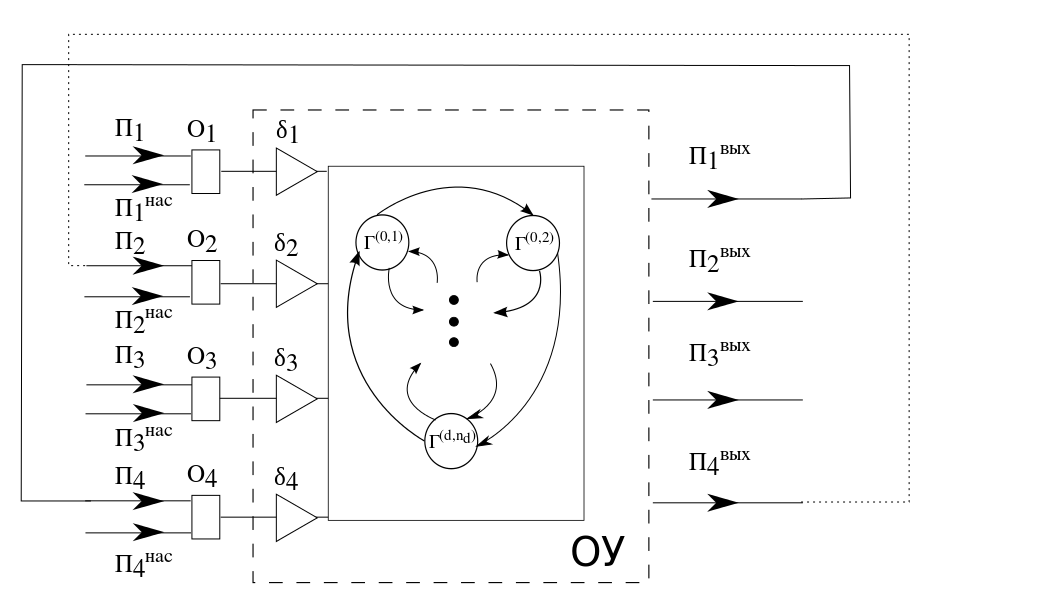
\includegraphics[scale=0.5]{SystemScheme.png} 
\caption{Структурная схема системы обслуживания}
\label{SystemScheme}
\end{figure}

Пусть в систему с одним обслуживающим устройством поступают потоки $\Pi_1$, $\Pi_2$, $\Pi_3$  и $\Pi_4$. Требования по потоку $\Pi_j$ становятся в соответствующую очередь $O_j$ с неограниченной вместимостью, $j\in \{1, 2, 3, 4\}$. Для $j \in \{1, 2, 3\}$ дисциплина очереди $O_j$, поддерживаемая устройством $\delta_j$, имеет тип FIFO (First In First Out). Таким образом, для обслуживания из соответствующей очереди выбирается то требование, которое пришло раньше. Дисциплина очереди $O_4$ будет описана ниже. Входные потоки $\Pi_1$ и $\Pi_3$ формируются внешней средой, которая, будем предполагать, имеет только одно состояние, то есть вероятностная структура потоков не меняется с течением времени. Требования потоков $\Pi_1$ и $\Pi_3$ формируют независимые между собой неординарные пуассоновские потоки, то есть  стационарные, без последействия и ординарные потоки групп требований. Интенсивности соответствующих простейших потоков для $\Pi_1$ и $\Pi_3$ будем обозначать $\la_1$ и $\la_3$, а распределение числа заявок в группе по потоку $\Pi_j$ будем описывать производящей функцией
\begin{equation}
f_j(z) = \sum_{\nu=1}^{\infty} p_{\nu}^{(j)} z ^{\nu}
\label{GeneratingFunc}
\end{equation}
которая предполагается аналитической при любом $z$ таком, что $|z|<(1+\varepsilon), \varepsilon > 0$. Величина $p_{\nu}^{(j)}$ определяет вероятность того, что по потоку $\Pi_j$ число требований в группе равно $\nu$, $j\in \{1,3\}$. Обслуженные требования потока $\Pi_1$ поступают на повторное обслуживание, формируя при этом поток $\Pi_4$. Потоки $\Pi_2$ и $\Pi_3$ являются конфликтными, что означает запрет на одновременное обслуживание требований этих потоков и, следовательно, исследование системы не может быть сведено к задаче с меньшим числом потоков. 
 
 В каждый момент времени обслуживающее устройство находится в одном из конечного множества состояний $\Gamma=\{\G^{(k,r)} \colon k=0,1,\ldots,d; r=1,2,\ldots n_k\}$ с заданными натуральными числами $d$, $n_0$, $n_1$, $\ldots$, $n_d$. В каждом состоянии $\ga{k,r}$ обслуживающее устройство находится в течение времени $\Tt{k,r}$. Введем множества $\G^{\mathrm{I}}$, $\G^{\mathrm{II}}$, $\G^{\mathrm{III}}$ и $\G^{\mathrm{IV}}$ следующим образом. В состоянии $\gamma \in \G^{\mathrm{\Rmnum{1}}}$ обслуживаются только требования из очередей $O_1$, $O_2$ и $O_4$.
В состоянии $\gamma \in \G^{\mathrm{\Rmnum{2}}}$ обслуживаются только требования из очередей $O_2$ и $O_4$.
В состоянии $\gamma \in \G^{\mathrm{\Rmnum{3}}}$ обслуживаются только требования из очередей $O_1$, $O_3$ и $O_4$.
В состоянии $\gamma \in \G^{\mathrm{\Rmnum{4}}}$ обслуживаются только требования из очередей $O_3$ и $O_4$.
Тогда множество $\G$ есть объединение $\G = \G^{\mathrm{I}} \cup \G^{\mathrm{II}} \cup \G^{\mathrm{III}} \cup \G^{\mathrm{III}}$ непересекающихся подмножеств. Также в дальнейшем нам понадобятся множества ${}^1\G=\G^{\mathrm{\Rmnum{1}}} \cup \G^{\mathrm{\Rmnum{3}}}$, 
${}^2\G=\G^{\mathrm{\Rmnum{1}}} \cup \G^{\mathrm{\Rmnum{2}}}$,
${}^3\G=\G^{\mathrm{\Rmnum{3}}} \cup \G^{\mathrm{\Rmnum{4}}}$. 

Смена состояний обслуживающего устройства осуществляется по следующему правилу. Множество состояний $C_k = \{\G^{(k,r)} \colon r=1,2,\ldots n_k\}$ будем называть $k$-м циклом, $k=1$, $2$, $\ldots$, $d$ (Рис. \ref{GraphScheme}). При $k=0$ состояние вида $\ga{0,r}$ будем называть состоянием продления, $r=0$, $1$, $\ldots$, $n_0$. Положим $r \oplus_k 1 = r+1$ для $r<n_k$ и $r \oplus_k 1 = 1$ при $r=n_k$, $k = 0$, $1$, $\ldots$, $d$. В цикле $C_k$ выделим подмножества $C_k^{\mathrm{O}}$ выходных, $C_k^{\mathrm{I}}$ входных и $C_k^{\mathrm{N}} = C_k \setminus (C_k^{\mathrm{O}} \cup C_k^{\mathrm{I}})$ нейтральных состояний. Тогда после состояния $\ga{k,r} \hm\in C_k\setminus C_k^{\mathrm{O}}$ обслуживающее устройство переходит в состояние $\ga{k,r \oplus_k 1}$ того же цикла $C_k$. При $\ga{k,r}$ принадлежащем множеству $C_k^{\mathrm{O}}$ прибор переходит в состояние $\ga{k,r\oplus_k 1}$, если число требований в очереди $O_3$ в момент переключения больше заданного порога $L$. В противном случае, то есть если число требований в очереди $O_3$ меньше либо равно $L$, то новое состояние прибора будет состоянием продления $\ga{0,r_1}$, где $r_1=h_1(\ga{k,r})$ и $h_1(\cdot)$~--- заданное отображение множества $\bigcup\limits_{k=1}^d C_k^{\mathrm{O}}$ во множество $\{1,2,\ldots, n_0\}$. После состояния $\ga{0,r}$ выбирается состояние того же вида $\ga{0,r_2}$, если число требований в очереди $O_3$ меньше или равно $L$, где $r_2=h_2(r)$ и $h_2(\cdot)$~--- заданное отображение множества $\{1,2, \ldots, n_0\}$ на себя; в противном случае включается входное состояние $\ga{k,r_3} \in C_k^{\mathrm{I}}$, где $\ga{k,r_3}=h_3(r)$ и $h_3(\cdot)$~--- заданное отображение множества $\{1,2, \ldots, n_0\}$ на множество  $\bigcup\limits_{k=1}^d C_k^{\mathrm{I}}$. Считается, что все состояния продления $\ga{0,r}$ принадлежат множеству ${}^2 \G$, а также верны соотношения $C_k^\mathrm{O}\subset {}^2 \G$ и $C_k^\mathrm{I}\subset {}^3 \G$.

\begin{figure}[hb]\centering
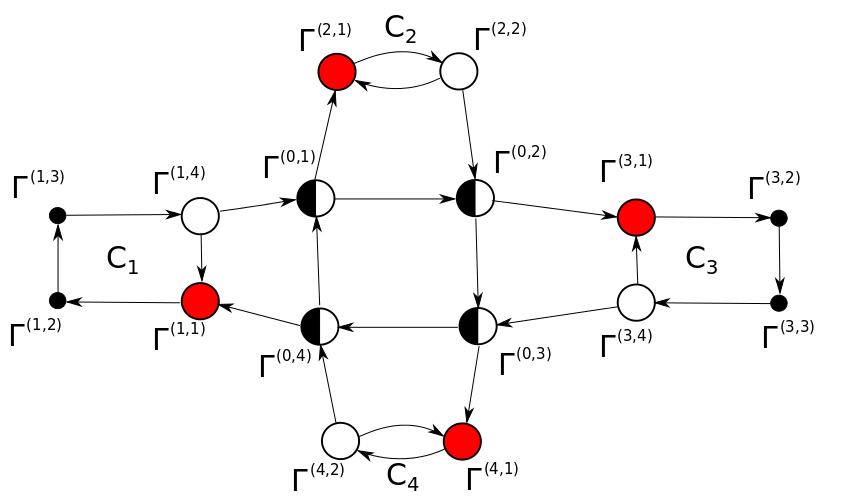
\includegraphics[scale=0.5]{GraphScheme3.png} 
\caption{Класс графов переходов. Незакрашенные вершины являются выходными вершинами, красным отмечены входные вершины, черным --- нейтральные, наполовину закрашенным вершинам соответствуют состояния продления}
\label{GraphScheme}
\end{figure}
%\subsection{Допустимые графы переходов состояний ОУ}

Таким образом, смена состояний обслуживающего устройства задается соотношением:
\begin{equation}
h(\ga{k,r},x) = 
\begin{cases}
\ga{k,r\oplus_k 1},& \quad \text{ если } \ga{k,r}\in C_k\setminus C_k^{\mathrm{O}};\\
\ga{k,r\oplus_k 1},& \quad \text{ если } \ga{k,r}\in C_k^{\mathrm{O}} \text{ и } x>L;\\
\ga{k,h_1(\ga{k,r})},& \quad \text{ если } \ga{k,r}\in C_k^{\mathrm{O}} \text{ и } x\leqslant L;\\
\ga{0,h_2(r)},& \quad \text{ если } k=0 \text{ и } x\leqslant L;\\
h_3(r),& \quad \text{ если } k=0 \text{ и } x > L.
\end{cases}
\label{hLaw}
\end{equation}

Рассмотрим введеные обозначения на примере Рис.~\ref{GraphScheme}. Примерами входных состояний являются $\ga{1,1} \in C_1^{\mathrm{I}}$ и $\ga{2,3} \in C_2^{\mathrm{I}}$, выходных состояний~--- $\ga{1,4} \in C_1^{\mathrm{O}}$ и $\ga{2,1} \in C_2^{\mathrm{O}}$, нейтральных состояний~--- $\ga{1,2}, \ga{1,3}, \ga{1,n_1} \in C_1^{\mathrm{N}}$ и $\ga{2,2} \in C_2^{\mathrm{N}}$. Состояния продления представлены на графе вершинами $\ga{0,1}$, $\ga{0,2}$, $\ga{0,3}$ и $\ga{0,4}$. Далее, отображение $h_1(\cdot)$ на графе задано таким образом, что оно переводит, например, выходное состояние $\ga{1,4}$ в число $1$~--- номер состояния продления $\ga{0,1}$, то есть $h_1(\ga{1,4})=1$. Аналогично $h_2(1)=2$, $h_2(2)=4$ и $h_2(3)=1$. Примером отображения $h_3(\cdot)$ является $h_3(2)=\ga{2,3}$.


Предполагается, что длительности обслуживания различных требований могут быть зависимыми и иметь различные законы распределения, поэтому вместо классического способа, состоящего в указании функции распределения длительности обслуживания произвольного требования, будут использованы потоки насыщения. Потоки насыщения $\Pi^{\mathrm{\text{нас}}}_j$, $j \in \{1,2,3,4\}$, определяются как виртуальные выходные потоки при 
условии максимального использования ресурсов обслуживающего устройства, а для $j\in \{1, 2, 3\}$ еще и при условии максимальной загрузки соответствующих очередей. Поток насыщения $\Pi^{\mathrm{\text{нас}}}_j$, $j\in \{1,2,3\}$, будет содержать неслучайное число $\ell_{k,r,j}$ требований, обслуженных в течение времени $\Tt{k,r}$, если $\ga{k,r} \in~^j\G$, и будет содержать $0$ требований в противном случае: $\ga{k,r} \notin ~^j\G$. Пусть $Z_+$~--- множество целых неотрицательных чисел. Тогда, при условии, что в очереди $O_4$ находится $x \in Z_+$ требований, поток насыщения $\Pi^{\mathrm{\text{нас}}}_4$ определим как поток, содержащий все $x$ требований.
%\subsection{Пример: тандем из двух перекрестков} 
Наконец, при состоянии обслуживающего устройства $\ga{k,r}$ каждое требование из очереди $O_4$ с вероятностью $p_{k,r}$ и независимо от других завершает обслуживание и отправляется в очередь $O_2$ потока~$\Pi_2$. С вероятностью $1-p_{k,r}$ требование очереди $O_4$ остается в ней до следующего такта. На следующем такте процесс повторяется.

В качестве наглядной физической интерпретации можно привести тандем из двух перекрестков (рис. \ref{crossroads}).
\begin{figure}[h]
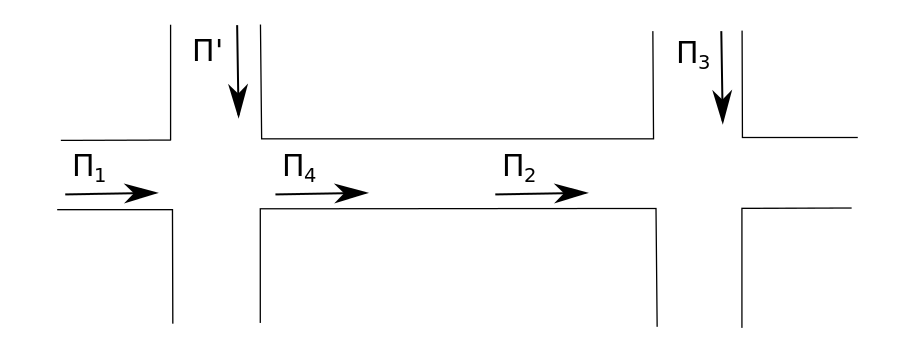
\includegraphics[scale=0.5]{Crossroads.png} 
\caption{Пример: тандем перекрестков}
\label{crossroads}
\end{figure}
В качестве потоков требований, формируемых внешней средой, выступают потоки прибывающих на перекрестки машин: конфликтные потоки $\Pi_1$, $\Pi_5$ на первом перекрестке, а также поток $\Pi_3$ на втором. Каждая машина из потока $\Pi_1$, проезжая первый перекресток, становится в очередь $O_4$ потока $\Pi_4$ и затем с некой вероятностью ($p_{k,r}$ для состояния $\ga{k,r}$ обслуживающего устройства) доезжает до следующего перекрестка, или же не успевает это сделать и остается в очереди $O_4$ до следующего такта обслуживания. В случае, если машина из очереди $O_4$ успевает доехать до второго перекрестка, она становится в очередь $O_2$ и ждет своей очереди для его прохождения.

Предполагается, что светофор на первом перекрестке имеет лишь два состояния $\{g_{1,1},g_{1,2}\}$: в состоянии $g_{1,1}$ машины потока $\Pi_1$ пропускаются фиксированное количество времени $\widetilde T^{(1,1)}$ (<<зеленый>> свет для $\Pi_1$); в состоянии $g_{1,2}$ --- простаивают в течение времени $\widetilde T^{(1,2)}$ (<<красный>> свет для $\Pi_1$). Светофор на втором перекрестке обслуживает по алгоритму с продлением: дополнительно к состоянию обслуживания потока $\Pi_3$ (состояние $g_{2,1}$), также имеется два состояния обслуживания потока $\Pi_2$ (состояния $\{g_{2,2},g_{2,3}\}$). Первое из них включается всегда после завершения обслуживания потока $\Pi_3$, а второе включается, если после очередного такта обслуживания потока $\Pi_2$ длина очереди $O_3$ не превосходит уровня $L$.
Длительности пребывания светофора на втором перекрестке в каждом из состояний суть $\widetilde T^{(2,1)}$, $\widetilde T^{(2,2)}$ и $\widetilde T^{(2,3)}$.


Рассматривая тандем из двух перекрестков как единую систему массового обслуживания и предполагая наблюдение за ней только в (дискретные) моменты переключения состояния хотя бы одного из светофоров, может быть показано, что количество различных состояний у полученной системы конечно. Действительно, положим, например, за состояние объединенной системы вектор $(g^{(1)},g^{(2)}, s, t)$, где $g^{(1)}\in \{g_{1,1},g_{1,2}\}$~--- состояние $1$--го перекрестка, $g^{(2)}\in \{g_{2,1},g_{2,2},g_{2,3}\}$~--- состояние $2$--го перекрестка, $s \in \{0, 1, 2\}$~--- номер последнего сменившего состояние перекрестка (принимает значение $0$ в случае, если сменили состояние оба перекрестка) и $t \in \{0, 1, 2, \ldots, T\}$~--- количество времени, оставшееся у продолжающего обслуживание с прошлого такта перекрестка (принимает значение $0$, если принимает значение $0$ величина $s$). Здесь $T$~--- максимальная длительность нахождения каждого из светофоров в одном состоянии. Тогда количество различных состояний не трудно посчитать и оно не будет превышать величины  $2\times 3 \times 3 \times T$.

В завершение построения примера отметим, что при прохождении перекрестков машины предполагаются движущимися только в прямом направлении, то есть перемешивания конфликтных потоков не допускается. Таким образом, поток $\Pi_5$ не представляет интереса для дальнейшего исследования системы и может быть отброшен и, следовательно, построенный пример целиком удовлетворяет структурной схеме на рис. \ref{SystemScheme}.

Теперь продемонстрируем на конкретном числовом примере выделение циклов и состояний продления. Пусть изменение состояний перекрестков и время пребывания (в секундах для определнности) в каждом из состояний задается графами на рис. \ref{SystemStates}.
\begin{figure}[h]
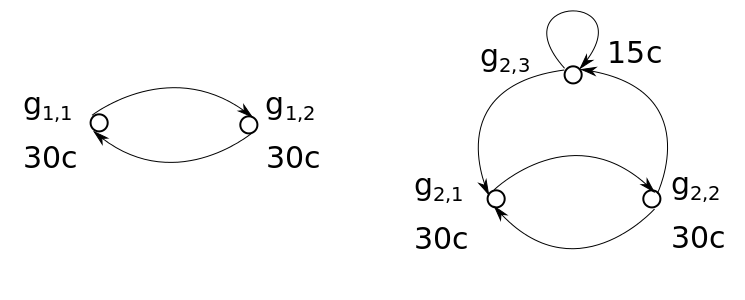
\includegraphics[scale=0.5]{SystemStates.png} 
\caption{Числовой пример тандема перекрестков. Левый граф соответствует первому перекрестку, правый~--- второму}
\label{SystemStates}
\end{figure}
За начальное состояние объединенной системы примем $\G_0=(g_{1,1},g_{2,1},0,0)$, то есть первый перекресток находится в состоянии $g_{1,1}$, второй~--- в состоянии $g_{2,1}$, и оба только начали свою работу в своем состоянии (этот факт моделируется равенствами $s=0$ и $t=0$). Следующая смена состояний случится у обоих перекрестков одновременно и приведет к следующему состоянию $(g_{1,2},g_{2,2}, 0, 0)$. Далее смена состояний произойдет также у первого и второго перекрестков, однако второй перекресток может перейти как в состояние $g_{2,1}$, так и в состояние продления $g_{2,3}$. Таким образом следущим состоянием тандема будет либо опять $(g_{1,1},g_{2,1},0,0)$, либо $(g_{1,1},g_{2,3},0,0)$. Продолжая рассуждения аналогичным образом, получим следущий список всех возможных состояний системы:
\begin{align*}
(g_{1,1},g_{2,1},0,0)&=\ga{1,1} ,& \quad (g_{1,2},g_{2,2},0,0)&=\ga{1,2} ,& \quad (g_{1,1},g_{2,3},0,0)&=\ga{0,1}, \\
(g_{1,1},g_{2,3},15,2)&=\ga{0,2} ,& \quad (g_{1,2},g_{2,3},0,0)&=\ga{0,3} ,& \quad (g_{1,2},g_{2,3},15,2)&=\ga{0,4}, \\
(g_{1,2},g_{2,1},15,2)&=\ga{4,1} ,& \quad (g_{1,1},g_{2,1},15,1)&=\ga{4,2} ,& \quad (g_{1,1},g_{2,2},15,2)&=\ga{4,3}, \\
(g_{1,2},g_{2,2},15,1)&=\ga{4,4} ,& \quad (g_{1,2},g_{2,3},15,2)&=\ga{0,5} ,& \quad (g_{1,2},g_{2,1},0,0)&=\ga{3,1}, \\
(g_{1,1},g_{2,2},0,0)&=\ga{3,2} ,& \quad (g_{1,1},g_{2,1},15,2)&=\ga{2,1} ,& \quad (g_{1,2},g_{2,1},15,1)&=\ga{2,2}, \\
(g_{1,2},g_{2,2},15,2)&=\ga{2,3} ,& \quad (g_{1,1},g_{2,2},15,1)&=\ga{2,4}. & &
\end{align*}
В соответсвии с приведенными выше обозначениями, множества $C_1$, $C_2$, $C_3$, $C_4$, а также множество состояний продления строятся однозначным образом. Множествами входных состояний будут $C_1^{\mathrm{I}}=\{\ga{1,1}\}$, $C_2^{\mathrm{I}}=\{\ga{2,1}\}$, $C_3^{\mathrm{I}}=\{\ga{3,1}\}$ и $C_4^{\mathrm{I}}=\{\ga{4,1}\}$. Множествами выходных состояний будут $C_1^{\mathrm{O}}=\{\ga{1,2}\}$, $C_2^{\mathrm{O}}=\{\ga{2,4}\}$, $C_3^{\mathrm{O}}=\{\ga{3,2}\}$ и $C_4^{\mathrm{O}}=\{\ga{4,4}\}$. Функции $h_1(\cdot)$, $h_2(\cdot)$ и $h_3(\cdot)$ задаются поточечно:
\begin{equation*}
h_1(\ga{1,2})=1, \quad h_1(\ga{2,4})=2, \quad h_1(\ga{3,2})=3, \quad h_1(\ga{4,4})=5,
\end{equation*}
\begin{equation*}
h_2(1)=2, \quad h_2(2)=3, \quad h_2(3)=4 \quad h_2(4)=1, \quad h_2(5)=1,
\end{equation*}
\begin{equation*}
h_3(1)=\ga{2,1}, \quad h_3(2)=\ga{3,1}, \quad h_3(3)=\ga{4,1} \quad h_3(4)=\ga{1,1}, \quad h_3(5)=\ga{1,1}.
\end{equation*}
Этим завершается построение числового примера.

\subsection{Представление рассматриваемой системы обслуживания в виде кибернетической управляющей системы}
Описанная в предыдущем разделе на содержательном уровне система массового обслуживания должна рассматриваться как кибернетическая управляющая система обслуживания (см. \cite{Zorine:2011}). Схема управляющей системы приведена на рис. \ref{SystemScheme}. На схеме присутствуют следующие блоки: 1) внешняя среда с одним состоянием; 2) входные полюса первого типа~--- входные потоки $\Pi_1$, $\Pi_2$, $\Pi_3$, $\Pi_4$; 3) входные полюса второго типа~--- потоки насыщения $\Pi_1^{\mathrm{\text{нас}}}$, $\Pi_2^{\mathrm{\text{нас}}}$, $\Pi_3^{\mathrm{\text{нас}}}$, $\Pi_4^{\mathrm{\text{нас}}}$; 4) внешняя память~--- очереди $O_1$, $O_2$, $O_3$, $O_4$; 5) устройство по переработкe информации внешней памяти~--- устройства по поддержанию дисциплины очереди $\delta_1$, $\delta_2$, $\delta_3$, $\delta_4$; 6) внутренняя память обслуживающего устройства~--- обслуживающее устройство (ОУ); 7) устройство по переработке информации во внутренней памяти~--- граф смены состояний; 8) выходные полюса $\Pi_1^{\mathrm{\text{вых}}}$, $\Pi_2^{\mathrm{\text{вых}}}$, $\Pi_3^{\mathrm{\text{вых}}}$, $\Pi_4^{\mathrm{\text{вых}}}$. Координатой блока является номер этого блока на схеме. 

Для задания информации блоков введем следующие величины и элементы, а также укажем множества их возможных значений. В качестве дискретной временной шкалы выберем последовательность $\tau_0=0$, $\tau_1$, $\tau_2$, $\ldots$ моментов смены состояний обслуживающего устройства. Обозначим $\G_i$ из множества $\G$ состояние обслуживающего устройства в течение времени $\left(\tau_{i-1};\tau_i\right]$, количество $\vk_{j,i} \in Z_+ $ требований в очереди $O_j$ в момент времени $\tau_i$, количество $\eta_{j,i} \in Z_+$ требований, поступивших в очередь $O_j$ по потоку $\Pi_j$ в течение времени $\left(\tau_{i};\tau_{i+1}\right]$, количество $\xi_{j,i} \in Z_+$ требований по потоку насыщения $\Pi^{\mathrm{\text{нас}}}_j$ в течение времени $\left(\tau_{i};\tau_{i+1}\right]$, количество $\overline{\xi}_{j,i}\in Z_+$ реально обслуженных требований по потоку $\Pi_j$ в течение времени $\left(\tau_{i};\tau_{i+1}\right]$, $j\in \{1,2,3,4\}$.

Закон изменения состояния обслуживающего устройства будем предполагать заданным соотношением 
\begin{equation}
\G_{i+1}=h(\G_i,\vk_{3,i}),
\label{gammaFunc}
\end{equation}
где отображение $h(\cdot,\cdot)$ определено в \eqref{hLaw}.
Для определения длительности $T_{i+1}$ состояния обслуживающего устройства в течение времени $\left(\tau_{i};\tau_{i+1}\right]$ удобно ввести функцию $h_T(\cdot,\cdot)$:
\begin{equation*}
T_{i+1}=h_T(\G_i,\vk_{3,i})= \Tt{k,r},\quad  \text{ где } \ga{k,r}=\G_{i+1}=h(\G_i,\vk_{3,i}).
%\label{timeLaw}
\end{equation*}
Функциональная зависимость
\begin{equation}
\overline{\xi}_{j,i}=\min\{\vk_{j,i}+\eta_{j,i},\xi_{j,i}\}, \quad j\in \{1,2,3\},
\label{saturationEq}
\end{equation}
между величиной $\overline{\xi}_{j,i}$ и величинами $\vk_{j,i}$, $\eta_{j,i}$, $\xi_{j,i}$ реализует стратегию механизма обслуживания требований. Далее, поскольку 
\begin{equation*}
\vk_{j,i+1}=\vk_{j,i}+\eta_{j,i}-\overline{\xi}_{j,i}, \quad  j\in \{1,2,3\},
\end{equation*}
то из \eqref{saturationEq} следует соотношение
\begin{equation}
\vk_{j,i+1}=\max\{{0,\vk_{j,i}+\eta_{j,i}-\xi_{j,i}}\}, \quad j\in \{1,2,3\}.
\label{queuesFunc}
\end{equation}
Из формулировки поставленной задачи (см. также структурную схему на рис.~\ref{SystemScheme}) следуют соотношения для потока $\Pi_4$:
\begin{equation}
\eta_{4,i} = \min\{\xi_{1,i}, \vk_{1,i}+\eta_{1,i}\}, \quad \vk_{4,i+1}=\vk_{4,i}+\eta_{4,i}-\eta_{2,i}, \quad \xi_{4,i} = \vk_{4,i}.
\label{FourthFunc}
\end{equation}

Нелокальное описание входных потоков и потоков насыщения состоит в указании некоторых свойств условных распределений выделенных дискретных компонент $\eta_i=(\eta_{1,i},\eta_{2,i}, \eta_{3,i}, \eta_{4,i})$ и $\xi_i=(\xi_{1,i}, \xi_{2,i}, \xi_{3,i}, \xi_{4,i})$ маркированных точечных процессов \linebreak $\{(\tau_i, \nu_i, \eta_i); i\geqslant 0\}$ и $\{(\tau_i, \nu_i, \xi_i); i\geqslant 0\}$ при фиксированных значениях метки $\nu_i = (\Gamma_i;\vk_{1,i},\vk_{2,i},\vk_{3,i},\vk_{4,i})$. 
Введем функции $\vp_1(\cdot,\cdot)$, $\vp_3(\cdot,\cdot)$ из разложений 
\begin{equation*}
\sum_{x=0}^{\infty} z^x\vp_j(x,t) = \exp\{\la_j t (f_j(z)-1)\},
\end{equation*}
где $f_j(z)$ определены в \eqref{GeneratingFunc}, $j \in \{1,3\}$. Функция $\vp_j(x,t)$ есть вероятность поступления $x=0$, $1$, $\ldots$ требований по потоку $\Pi_j$ за время $t \geqslant 0$. Положим $\vp_j(x,t)$ равной нулю при $x < 0$. Функцию $\psi(\cdot,\cdot,\cdot)$ зададим формулой
\begin{equation*}
\psi(k;x,u)=C_x^k u^k (1-u)^{x-k}.
\end{equation*}
По своему смыслу $\psi(k;x,u)$ есть вероятность поступления $k$ требований по потоку $\Pi_2$ при условии, что очередь $O_4$ содержит $x$ требований и обслуживающее устройство находится в состоянии $\ga{k,r}$, так что $u=p_{k,r}$. При нарушении условия $ 0\leqslant k \leqslant x$ положим $\psi(k;x,u)$ равной нулю.

Пусть $a=(a_1, a_2, a_3, a_4) \in Z_+^4$ и $x=(x_1, x_2, x_3, x_4) \in Z_+^4$. Тогда из постановки задачи на содержательном уровне следует, что при фиксированном значении метки $\nu_i=(\ga{k,r}; x_1, x_2, x_3, x_4)$ вероятность $\vp(a,k,r,x)$ одновременного выполнения равенств $\eta_{1,i}=a_1$, $\eta_{2,i}=a_2$, $\eta_{3,i}=a_3$, $\eta_{4,i}=a_4$ есть 
\begin{equation}
\vp_1(a_1,h_T(\ga{{k},{r}},x_3)) \times \psi(a_2,x_2, p_{\tilde{k},\tilde{r}}) \times \vp_3(a_3,h_T(\ga{{k},{r}},x_3))
\times \delta_{a_4,\min{\{\tilde{\ell}(\tilde{k},\tilde{r},1), x_1+a_1}\}},
\label{conditionProbOne}
\end{equation}
где $0\leqslant a_2\leqslant x_2$, $\ga{\tilde{k},\tilde{r}}=h(\ga{k,r},x_3)$,  $\delta_{i,j}$ есть символ Кронекера
\begin{equation*}
\delta_{i,j}=\begin{cases} 1, \quad \text{ если }i=j\\0, \quad \text{ если } i\neq j,
\end{cases},
\end{equation*}
и для $j\in \{1, 2, 3\}$
\begin{equation*}
\widetilde{\ell}(k,r,j)=\begin{cases}
\ell_{k,r,j},& \quad \text{если } \ga{k,r} \in {}^j\G,\\
0,& \quad \text{если } \ga{k,r} \notin {}^j\G. \end{cases}
\end{equation*}
Пусть $b=(b_1, b_2, b_3, b_4)$. Из содержательной постановки задачи следует, что вероятность $\zeta(b, k, r, x)$ выполнения равенств $\xi_{1,i}=b_1$, $\xi_{2,i}=b_2$, $\xi_{3,i}=b_3$, $\xi_{4,i}=b_4$ при фиксированном значении метки $\nu_i=(\ga{k,r}; x_1, x_2, x_3, x_4)$ есть
\begin{equation}
\delta_{b_1,\tilde{\ell}(\tilde{k},\tilde{r},1)} \times \delta_{b_2,\tilde{\ell}(\tilde{k},\tilde{r},2)} \times 
\delta_{b_3,\tilde{\ell}(\tilde{k},\tilde{r},3)} \times \delta_{b_4,x_4}.
\label{conditionProbTwo}
\end{equation}
Из формулы \eqref{conditionProbTwo} следует для $j\in \{1, 2, 3\}$, что вероятность события $\xi_{j,i}=0$ равна $1$ в случае $h(\ga{k,r},x_3)\notin {}^j\G$ и что вероятность события $\xi_{j,i}=\ell_{\tilde{k},\tilde{r}}$ равна $1$, если $\ga{\tilde{k},\tilde{r}}=h(\ga{k,r},x_3)\in {}^j\G$.


Содержательный смысл следующей теоремы состоит в том, что сформулированные выше функциональные связи и вероятностные свойства введенных объектов непротиворечивы и могут быть реализованы на некотором общем вероятностном пространстве.
%Построим теперь 	вероятностное пространство $(\Omega, {\cal F}, \Pr(\cdot))$, чтобы можно было рассматривать введеные величины как случайные величины на этом пространстве. А именно, докажем следующую теорему.
\begin{theorem}
Пусть $\gamma_0=\ga{k,r} \in \G$ и $x_0=(x_{1,0},x_{2,0}, x_{3,0},x_{4,0})\in Z_+^4$ фиксированы.
Тогда существует вероятностное пространство $(\Omega, {\cal F}, \Pr(\cdot))$ и заданные на нем случайные величины $\eta_{j,i}=\eta_{j,i}(\omega)$, $\xi_{j,i}=\xi_{j,i}(\omega)$, $\overline{\xi}_{j,i}=\overline{\xi}_{j,i}(\omega)$,  $\vk_{j,i}=\vk_{j,i}(\omega)$ и случайные элементы $\G_i=\G_i(\omega)$, $i\geqslant 0$, $j\in \{1, 2, 3, 4\}$, такие, что $\G_0(\omega) = \gamma_0$ и $\vk_0(\omega)=x_0$, выполняются соотношения \eqref{gammaFunc}, \eqref{queuesFunc}, \eqref{FourthFunc} и для любых $a$, $b$, $x^t=(x_{1,t},x_{2,t},x_{3,t},x_{4,t}) \in Z_+^4$ и векторов $\eta_i=(\eta_{1,i}, \eta_{2,i}, \eta_{3,i}, \eta_{4,i})$, $\xi_i=(\xi_{1,i}, \xi_{2,i}, \xi_{3,i}, \xi_{4,i})$, $\vk_i=(\vk_{1,i}, \vk_{2,i}, \vk_{3,i}, \vk_{4,i})$ верно равенство
\begin{equation}
\Pr \left(\{ \omega \colon \eta_i = a, \xi_i=b\} \left|\bigcap_{t=0}^{i}\{\omega\colon \G_t=\ga{k_t,r_t}, \vk_t=x^t\}\right.\right)=
\vp(a,k_i,r_i,x^i)\times \zeta(b,k_i,r_i,x^i),
\label{ProbablititiesToProve}
\end{equation}
где функции $\vp(\cdot, \cdot, \cdot, \cdot)$ и $\zeta(\cdot, \cdot, \cdot, \cdot)$ определяются формулами \eqref{conditionProbOne} и \eqref{conditionProbTwo} соответственно.

\label{myTheorem}
\end{theorem}
\begin{proof}
В соответствии с теоремой Ионеску Тулчи (см. \cite{Shiryaev}) для доказательства достаточно задать на $(\Omega_0, {\cal F}_0)$ вероятностную меру $P_0(\cdot)$ и далее, считая для $0 < i \leqslant n$ и каждого набора элементарных исходов $(\omega_0, \omega_1, \ldots, \omega_{i-1})$ заданной на $(\Omega_i, {\cal F}_i)$ вероятностную меру $P(\omega_0,\omega_1,\ldots, \omega_{i-1};\cdot)$, задать на $(\Omega_{n+1}, {\cal F}_{n+1})$ меру $P(\omega_0,\omega_1,\ldots, \omega_{n};\cdot)$, причем для любого множества $B\in {\cal F}_i$ функции $P(\omega_0,\omega_1,\ldots, \omega_{i-1};B)$
должны быть измеримыми функциями от $(\omega_0, \omega_1, \ldots, \omega_{i-1})$. Тогда для $\Omega=\prod\limits_{i=0}^{\infty}\Omega_i$ и ${\cal F}=\bigotimes\limits_{i=0}^{\infty} {\cal F}_i$ на $(\Omega,{\cal F})$ будет существовать единственная вероятностная мера $\Pr(\cdot)$ такая, что для любого $i \geqslant 0$ верно равенство
\begin{equation}
\Pr\{\omega \colon \omega_0 \in A_0, \omega_1 \in A_1, \ldots, \omega_i\in A_i\} = P_i(A_0 \times A_1 \times \ldots \times A_i),
\label{ProbabilitiesGeneral}
\end{equation}
где 
\begin{equation}
 P_i(A_0 \times A_1 \times \ldots \times A_i) = \int_{A_0} P_0(d \omega_0) \int_{A_1} P(\omega_0;d \omega_1) \ldots \int_{A_i} P(\omega_0, \omega_1, \ldots, \omega_{i-1}; d \omega_i),
\label{ProbabilitiesGeneralOne}
\end{equation}
для любого $A_i$ из ${\cal F}_i$. 

Итак, за описание элементарного исхода $\omega_i \in \Omega_i$ для произвольного $i \geqslant 0$ примем набор $\omega_i=(\omega_{1,i},\omega_{2,i},\omega_{3,i})$, $\omega_{j,i}\in Z_+$. Таким образом, $\Omega_i=Z_+^3$ и в качестве $\sigma$-алгебры ${\cal F}_i$ возьмем множество всех подмножеств множества $\Omega_i$: ${\cal F}_i=2^{\Omega_i}$. Пусть $\ga{\widetilde{k},\widetilde{r}}=h(\ga{k,r},x_{3,0})$. Тогда  поскольку множество $\Omega_0$ счетно, определим вероятностную меру $P_0(\cdot)$ на измеримом пространстве $(\Omega_0,{\cal F}_0)$ ее значениями на одноточечных множествах:
\begin{equation}
P_0(\{(a_1,a_2,a_3)\})=\vp_1(a_1,h_T(\ga{k,r})) \times \psi(a_2,x_{2,0}, p_{\tilde{k},\tilde{r}}) \times \vp_2(a_1,h_T(\ga{k,r})).
\label{probabilitiesOne}
\end{equation}
Для $j\in \{1,2,3\}$ определим величины
\begin{equation}
\G_0=\gamma_0, \quad \vk_{j,0}=x_{j,0}, \quad \xi_{j,0}(\omega_0)=\widetilde{l}(\tilde{k},\tilde{r},j), \quad \eta_{j,0}=\omega_{j,0},
\label{startRekOne}
\end{equation}
и
\begin{equation}
 \vk_{4,0}=x_{4,0}, \quad \xi_{4,0}=x_{4,0}, \quad \eta_{4,0}=\min\{\xi_{1,0}, x_{1,0}+\eta_{1,0}\}.
\label{startRekTwo}
\end{equation}
Теперь, предполагая заданными на $(\Omega_i, {\cal F}_i)$ вероятностные меры $P(\omega_0, \omega_1, \ldots, \omega_{i-1};\cdot)$, заданными величины $\G_i$, $\vk_{j,i}$, $\xi_{j,i}$, $\eta_{j,i}$, $i\in \{0,1,\ldots,n\}$, $j\in \{1, 2, 3, 4\}$ и фиксируя набор $(\omega_0, \omega_1, \ldots, \omega_{n})$, определим на $(\Omega_{n+1}, {\cal F}_{n+1})$ меру $P(\omega_0, \omega_1, \ldots, \omega_n;\cdot)$. Положим для $j\in \{1, 2, 3\}$
\begin{equation}
\G_{n+1}=\ga{k^*,r^*}=h(\G_{n},\vk_{3,n}), \quad \vk_{j,n+1}=\max\{ 0,\vk_{j,n}+\eta_{j,n} -\xi_{j,n}\},
\label{NextRekOne}
\end{equation}
\begin{equation}
\vk_{4,n+1}=\vk_{4,n}+\eta_{4,n}-\eta_{2,n}, \quad \xi_{j,n+1}=\widetilde{l}(k^*,r^*,j),
\label{NextRekTwo}
\end{equation}
\begin{equation}
\eta_{j,n+1}=\omega_{j,n+1}, \quad \eta_{4,n+1}=\min\{\xi_{1,n+1}, \vk_{1,n+1}+\eta_{1,n+1}\}, \quad \xi_{4,n+1}=\vk_{4,n+1}.
\label{NextRekThree}
\end{equation}
Тогда, по аналогии с построением вероятностной меры $P_0(\cdot)$, зададим меру $P(\omega_0,\omega_1,\ldots,\omega_n;\cdot)$ на одноточечных множествах $\{(a_1,a_2,a_3)\}$:
\ml
{
P(\omega_0,\omega_1,\ldots,\omega_n;\{(a_1,a_2,a_3)\}) = \\
= \vp_1(a_1,h_T(\G_n,x_{3,n})) \times \psi(a_2,x_{2,n}, p_{k^*,r^*}) \times \vp_2(a_3,h_T(\G_n,x_{3,n})).
\label{probabilitiesTwo}
}
Вероятностное пространство $(\Omega,{\cal F},\Pr(\cdot))$ построено. 

Теперь докажем, что введеные с помощью \eqref{startRekOne}~--~\eqref{NextRekThree} случайные элементы $\G_i(\omega)$ и случайные величины $\vk_{j,i}(\omega)$, $\eta_{j,i}(\omega)$, $\xi_{j,i}(\omega)$, $i \geqslant 0$, $j \in \{1, 2, 3, 4\}$ удовлетворяют условиям теоремы. Из формулы \eqref{NextRekOne} следует, что случайные элементы $\G_i$ удовлетворяют соотношению \eqref{gammaFunc}, а случайные величины $\vk_{j,i}$ для $j\in \{1, 2, 3\}$ удовлетворяют соотношению \eqref{queuesFunc}. Из формулы \eqref{NextRekTwo} заключаем, что $\vk_{4,i}$ удовлетворяет $\eqref{FourthFunc}$. Далее, из \eqref{startRekTwo} и \eqref{NextRekThree} следует справедливость соотношений \eqref{FourthFunc} для величин $\eta_{4,i}$ и $\xi_{4,i}$. 

Перейдем к доказательству равенства \eqref{ProbablititiesToProve}. Для этого найдем явное выражение для условной вероятности $\Pr (\{ \omega \colon \eta_i = a, \xi_i=b\} | \bigcap_{t=0}^{i}\{\omega\colon \G_t=\ga{k_t,r_t}, \vk_t=x^t\})$. Пусть $\ga{\tilde{k}_i,\tilde{r}_i}=h(\ga{k_i,r_i},x^i)$. Распишем по определению условной вероятности:
\ml
{
\Pr \left(\left\{ \omega \colon \eta_i = a, \xi_i=b\right\}  \left| \bigcap_{t=0}^{i}\left\{\omega\colon \G_t=\ga{k_t,r_t}, \vk_t=x^t\right\}\right.\right) = \\
=\Pr\left(\{ \omega \colon \eta_i = a, \xi_i=b \} \cap \bigcap_{t=0}^{i}\{\omega\colon \G_t=\ga{k_t,r_t}, \vk_t=x^t\}\right) \Big/
\Pr\left( \bigcap_{t=0}^{i}\{\omega\colon \G_t=\ga{k_t,r_t}, \vk_t=x^t\}\right).
\label{Construction:1}
}
Далее из \eqref{ProbabilitiesGeneral}, \eqref{ProbabilitiesGeneralOne} и того факта, что $\G_i$ и $\vk_{i}$ не зависят от $\omega_i$ (этот факт следует из \eqref{startRekOne}~--~\eqref{NextRekTwo}), получим выражение для знаменателя последней дроби
\ml
{
\Pr\left( \bigcap_{t=0}^{i}\{\omega\colon \G_t=\ga{k_t,r_t}, \vk_t=x^t\}\right)=\\
=\sum_{\substack{\omega_0, \omega_1,\ldots \omega_{i-1} \colon \\ \G_t=\ga{k_t,r_t}, \vk_t=x^t, \forall 0\leqslant t \leqslant i-1}} P_0(\omega_0)\times P(\omega_0;\{\omega_1\})\times\ldots\times P(\omega_0,\omega_1,\ldots, \omega_{i-2};\{\omega_{i-1}\}).
\label{Construction:2}
}
Преобразуем множество $\{ \eta_i = a, \xi_i=b \} \cap \{\G_i=\ga{k_i,r_i}, \vk_i=x^i\}$, учитывая соотношения \eqref{startRekOne}~--~\eqref{NextRekThree}:
\mll
{
\left\{ \eta_i = a, \xi_i=b \right\} \cap \left\{\G_i=\ga{k_i,r_i}, \vk_i=x^i\right\} = \left\{\G_i=\ga{k_i,r_i}, \vk_i=x^i\right\} \cap\\
\cap \left\{ \eta_{j,i} = a_j, j\in \{1, 2, 3\}\right\} \cap \left\{ \xi_{j,i} = b_j, j\in \{1, 2, 3\}\right\} \cap \left\{ \xi_{4,i} = b_4 \right\} \cap  \left\{ \eta_{4,i} = a_4 \right\} = \\
= \left\{\G_i=\ga{k_i,r_i}, \vk_i=x^i\right\} \cap \left\{ \omega_{j,i} = a_j, j\in \{1, 2, 3\}\right\} \cap \left\{ b_j=\tilde{\ell}(\tilde{k}_i,\tilde{r}_i,j), j\in \{1, 2, 3\}\right\} \cap \\ 
\cap \left\{ b_4 = x_{4,i} \right\} \cap  \left\{ a_4=\min\left\{\tilde{\ell}(\tilde{k}_i,\tilde{r}_i,1), x_{1,i}+a_1\right\} \right\}. 
}
Тогда для числителя \eqref{Construction:1} имеем:
\ml
{
\Pr\left(\{ \omega \colon \eta_i = a, \xi_i=b \} \cap \bigcap_{t=0}^{i}\{\omega\colon \G_t=\ga{k_t,r_t}, \vk_t=x^t\}\right)=\\
= \Pr\left(\left\{ \eta_i = a, \xi_i=b \right\} \cap \left\{\G_i=\ga{k_i,r_i}, \vk_i=x^i\right\} \cap \bigcap_{t=0}^{i-1}\{\omega\colon \G_t=\ga{k_t,r_t}, \vk_t=x^t\}\right)=\\
= \delta_{b_4,x_{4,i}} \times \delta_{a_4,\min\left\{\tilde{\ell}(\tilde{k}_i,\tilde{r}_i,1), x_{1,i}+a_1\right\}} \times \prod_{j=1}^3\delta_{b_j,\tilde{\ell}(\tilde{k}_i,\tilde{r}_i,j)}   \times \\
\times \Pr\left( \left\{ \omega_{j,i} = a_j, j\in \{1, 2, 3\}\right\} \cap \left\{\G_i=\ga{k_i,r_i}, \vk_i=x^i\right\} \cap \bigcap_{t=0}^{i-1}\{\omega\colon \G_t=\ga{k_t,r_t}, \vk_t=x^t\}\right)
\label{Construction:3}
}
И по аналогии со знаменателем (см.~\eqref{Construction:2}), распишем последнюю вероятность:
\ml
{
\Pr\left( \left\{ \omega_{j,i} = a_j, j\in \{1, 2, 3\}\right\} \cap \left\{\G_i=\ga{k_i,r_i}, \vk_i=x^i\right\} \cap \bigcap_{t=0}^{i-1}\{\omega\colon \G_t=\ga{k_t,r_t}, \vk_t=x^t\}\right) =\\
= \sum_{\substack{\omega_0, \omega_1,\ldots \omega_{i-1} \colon \\ \G_t=\ga{k_t,r_t}, \vk_t=x^t, \forall 0\leqslant t \leqslant i-1}} P_0(\omega_0)\times P(\omega_0;\{\omega_1\})\times\ldots\times P(\omega_0,\omega_1,\ldots, \omega_{i-2};\{\omega_{i-1}\})\times\\
\times  P(\omega_0,\omega_1,\ldots, \omega_{i-1};\{(a_1, a_2, a_3)\}) = \\=
\vp_1(a_1,h_T(\G_n,x_{3,n})) \times \psi(a_2,x_{2,n}, p_{\tilde{k},\tilde{r}}) \times \vp_2(a_3,h_T(\G_n,x_{3,n})) \times \\ 
\times \sum_{\substack{\omega_0, \omega_1,\ldots \omega_{i-1} \colon \\ \G_t=\ga{k_t,r_t}, \vk_t=x^t, \forall 0\leqslant t \leqslant i-1}} P_0(\omega_0)\times P(\omega_0;\{\omega_1\})\times\ldots\times P(\omega_0,\omega_1,\ldots, \omega_{i-2};\{\omega_{i-1}\}).
\label{Construction:4}
}
Подставляя \eqref{Construction:2}, \eqref{Construction:3} и \eqref{Construction:4} в \eqref{Construction:1}, получим:
\mll
{
\Pr \left(\left\{ \omega \colon \eta_i = a, \xi_i=b\right\}  \left| \bigcap_{t=0}^{i}\left\{\omega\colon \G_t=\ga{k_t,r_t}, \vk_t=x^t\right\}\right.\right)  = \\
= \delta_{b_4,x_{4,i}} \times \delta_{a_4,\min\left\{\tilde{\ell}(\tilde{k}_i,\tilde{r}_i,1), x_{1,i}+a_1\right\}} \times \prod_{j=1}^3\delta_{b_j,\tilde{\ell}(\tilde{k}_i,\tilde{r}_i,j)} \times
\vp_1(a_1,h_T(\G_n,x_{3,n})) \times \\ \times \psi(a_2,x_{2,n}, p_{\tilde{k},\tilde{r}}) 
\times  \vp_2(a_3,h_T(\G_n,x_{3,n})) \times \\ 
\times \sum_{\substack{\omega_0, \omega_1,\ldots \omega_{i-1} \colon \\ \G_t=\ga{k_t,r_t}, \vk_t=x^t, \forall 0\leqslant t \leqslant i-1}} P_0(\omega_0)\times P(\omega_0;\{\omega_1\})\times\ldots\times P(\omega_0,\omega_1,\ldots, \omega_{i-2};\{\omega_{i-1}\}) \Big/ \\
\Big/ \sum_{\substack{\omega_0, \omega_1,\ldots \omega_{i-1} \colon \\ \G_t=\ga{k_t,r_t}, \vk_t=x^t, \forall 0\leqslant t \leqslant i-1}} P_0(\omega_0)\times P(\omega_0;\{\omega_1\})\times\ldots\times P(\omega_0,\omega_1,\ldots, \omega_{i-2};\{\omega_{i-1}\})
}
и после сокращения одинаковых сумм получаем в точности \eqref{ProbablititiesToProve}.
\end{proof}

\begin{corollary}
В условиях предыдущей теоремы верно равенство
\ml
{
\Pr \left(\{ \omega \colon \eta_i = a, \xi_i=b\} \left|\bigcap_{t=0}^{i}\{\omega\colon \G_t=\ga{k_t,r_t}, \vk_t=x^t\}\right.\right)=\\
=\Pr \left(\{ \omega \colon \eta_i = a, \xi_i=b\} \left|\{\omega\colon \G_i=\ga{k_i,r_i}, \vk_i=x^i\}\right.\right)
\label{eta:xi:forgetProperty}
}
\label{eta:xi:forget}
\end{corollary}
\begin{proof}
Действительно, из \eqref{ProbablititiesToProve} видно, что вероятность, стоящая в левой части равенства \eqref{eta:xi:forgetProperty}, равна величине $\vp(a,k_i,r_i,x^i)\times \zeta(b,k_i,r_i,x^i)$, зависящей только от значений $(\ga{k_i,r_i},x^i)$ пары $(\G_i,\vk_i)$ и не зависящей от значений остальных пар $(\G_t,\vk_t)_{0\leqslant t \leqslant i-1}$. Таким образом, знание о значениях пар $(\G_t,\vk_t)_{0\leqslant t \leqslant i-1}$ не влияет на значение вероятности $\Pr (\{ \omega \colon \eta_i = a, \xi_i=b\} |\bigcap_{t=0}^{i}\{\omega\colon \G_t=\ga{k_t,r_t}, \vk_t=x^t\})$, следовательно, \eqref{eta:xi:forgetProperty} верно.
\end{proof}
Таким образом, кибернетический подход позволил построить математическую модель управляющей системы обслуживания в виде последовательности случайных величин и случайных элементов, конструктивно заданных на некотором вероятностном пространстве. Выберем для дальнейшего исследования состояния обслуживающего устройства и длины всех очередей.

\subsection[Марковское свойство последовательности $\boldsymbol{\Mark}$]%
{Марковское свойство последовательности \\ $\boldsymbol{\Mark}$}

Теперь перейдем к вопросу о марковости последовательности $\Mark$. Введем следующие события:
\begin{equation}
A_i(k_i;r_i;x^i) = \{\G_i=\ga{k_i,r_i}\vk_i=x^i\}, \quad B_i(a;b) = \{\eta_i=a, \xi_i=b\}
\end{equation}
В новых обозначениях равенство \eqref{eta:xi:forgetProperty} перепишется следующим образом:
\begin{equation}
\Pr \left(B_i(a;b) \left| \bigcap_{t=0}^{i} A_t(k_t;r_t;x^t)\right.\right) = \Pr \left(B_i(a;b) \left|  A_i(k_i;r_i;x^i)\right.\right)
\label{new:notation:eta:xi:forget}
\end{equation}

Сформулируем и докажем теорему о марковости последовательности \linebreak$\Mark$.
\begin{theorem}
Пусть $\G_0=\ga{k,r}\in \G$ и $\vk_0=x^0\in Z_+^4$ фиксированы. Тогда последовательность $\Mark$ является однородной счетной цепью Маркова. 
\end{theorem}

\begin{proof}
Для доказательства достаточно показать, что 
\begin{equation}
\Pr \left( A_{i+1}(k_{i+1};r_{i+1};x^{i+1}) \left|\bigcap_{t=0}^{i} A_t(k_t;r_t;x^{t})\right.\right) = \Pr \left( A_{i+1}(k_{i+1};r_{i+1};x^{i+1}) \left|A_i(k_i;r_i;x^{i})\right.\right)
\label{markovToProve}
\end{equation}
Распишем левую часть равенства \eqref{markovToProve}. Учитывая то, что сумма $\cup_{a,b} B_i(a;b)$ по всем $a$ и $b$ из $Z_+^4$ непересекающихся событий $B_i(a;b)$ есть достоверное событие $=\Omega$, получим
\ml
{
\Pr \left( A_{i+1}(k_{i+1};r_{i+1};x^{i+1}) \left|\bigcap_{t=0}^{i} A_t(k_t;r_t;x^{t})\right.\right)  = \\
=\sum_{a,b}\Pr \left( A_{i+1}(k_{i+1};r_{i+1};x^{i+1})\cap B_i(a;b) \left|\bigcap_{t=0}^{i} A_t(k_t;r_t;x^{t})\right.\right) = \\
= \sum_{a,b}\Pr \left( B_i(a;b) \left|\bigcap_{t=0}^{i} A_t(k_t;r_t;x^{t})\right.\right)\times\\
\times \Pr \left( A_{i+1}(k_{i+1};r_{i+1};x^{i+1}) \left|B_i(a;b) \cap \bigcap_{t=0}^{i} A_t(k_t;r_t;x^{t})\right.\right)
\label{markovProof}
}
Из равенства \eqref{new:notation:eta:xi:forget} следует, что вероятность  $\Pr \left( B_i(a;b) \left|\bigcap_{t=0}^{i} A_t(k_t;r_t;x^{t})\right.\right)$ не зависит от предыстории $\bigcap_{t=0}^{i-1} A_t(k_t;r_t;x^{t})$. Далее, из соотношений \eqref{gammaFunc}, \eqref{queuesFunc} и \eqref{FourthFunc} можно заметить, что случайный элемент $\G_{i+1}$ и случайный вектор $\vk_{i+1}$ функционально выражается через $\G_i$, $\vk_i$, $\eta_i$ и $\xi_i$. Следовательно, вероятность $\Pr ( A_{i+1}(k_{i+1};r_{i+1};x^{i+1}) |B_i(a;b) \cap \bigcap_{t=0}^{i} A_t(k_t;r_t;x^{t}))$ не зависит от предыстории. Таким образом 
\begin{equation*}
\Pr \left( B_i(a;b) \left|\bigcap_{t=0}^{i} A_t(k_t;r_t;x^{t})\right.\right) = \\
\Pr \left( B_i(a;b) \left| A_i(k_i;r_i;x^{i})\right.\right)
\end{equation*}
и 
\mll
{
\Pr \left( A_{i+1}(k_{i+1};r_{i+1};x^{i+1}) \left|B_i(a;b) \cap \bigcap_{t=0}^{i} A_t(k_t;r_t;x^{t})\right.\right) = \\
=\Pr \left( A_{i+1}(k_{i+1};r_{i+1};x^{i+1}) \left|B_i(a;b) \cap A_i(k_i;r_i;x^{i})\right.\right)
}
откуда заключаем верность \eqref{markovToProve}.
\end{proof}

Убедившись в марковости последовательности $\Mark$, приведем формулу для вычисления ее переходных вероятностей.
\begin{theorem}
Пусть, как и раньше, $x$, $\tilde{x}\in Z_+^4$ и $\ga{k,r}$, $\ga{\tilde{k},\tilde{r}}=h(\ga{k,r},x_3) \in \G$. Тогда переходные вероятности однородной счетной марковской цепи $\Mark$ вычисляются по следующей формуле:
\begin{equation}
\P{\G_{i+1}=\ga{\tilde{k},\tilde{r}},\vk_{i+1}=\tilde{x}}{\G_{i}=\ga{k,r},\vk_i=x} 
= \vp(a,k,r,x),
\label{transitionToProve}
\end{equation}
где компоненты вектора $a$ находятся из соотношений
\begin{align}
a_j&=\tilde{x}_j-x_j+\tilde{\ell}(\tilde{k},\tilde{r},j), \quad j\in\{1, 2, 3\}\\
a_4&=\tilde{x}_4-x_4+\tilde{x_2}-x_2+\tilde{\ell}(\tilde{k},\tilde{r},2).
\end{align}
В случае, если $\ga{\tilde{k},\tilde{r}}\neq h(\ga{k,r},x_3)$, переходная вероятность равна нулю.
\end{theorem}
\begin{proof}
Для нахождения переходной вероятности $\Pr(\G_{i+1}=\ga{\tilde{k},\tilde{r}},\vk_{i+1}=\tilde{x}|\G_{i}=\ga{k,r},\vk_i=x) $ воспользуемся формулой полной вероятности. Выделим из множества событий вида $\{\eta_i=a;\xi_i=b\}$, $a$, $b\in Z_+^4$, полную группу несовместных событий, при условии наступления события $\{\G_{i}=\ga{k,r},\vk_i=x\}$, вероятности которых будут положительны. Из определения функций $\vp_j(x,t)$, $j\in \{1,3\}$, следует, что они положительны тогда и только тогда, когда $x \in Z_+^4$. Аналогично, $\psi(s,m,u)>0$ только в случае $0\leqslant s \leqslant m$. Тогда из формул \eqref{ProbablititiesToProve}, \eqref{conditionProbOne} и \eqref{conditionProbTwo} следует, что вероятность $\Pr(\eta_i=a, \xi_i=b|\G_{i}=\ga{k,r},\vk_i=x)$ положительна тогда и только тогда, когда 
\begin{equation}
b_4 = x_4, \quad b_j = \tilde{\ell}(\tilde{k},\tilde{r},j),\quad j\in\{1, 2, 3\},
\label{transitionB}
\end{equation}
и 
\begin{equation}
a_4=\min{\{\tilde{\ell}(\tilde{k},\tilde{r},1),x_1+a_1\}}, \quad  0\leqslant a_2 \leqslant x_4.
\label{transitionA}
\end{equation}
В следствии вышесказанного, распишем по формуле полной вероятности:
\mll
{
\P{\G_{i+1}=\ga{\tilde{k},\tilde{r}},\vk_{i+1}=\tilde{x}}{\G_{i}=\ga{k,r},\vk_i=x} = \\
= \sum_{\substack{a_1,a_3\in Z_+\\0\leqslant a_2 \leqslant x_4}} \P{\eta_i=a; \xi_i=b}{\G_{i}=\ga{k,r},\vk_i=x} \times \\ 
\times
\P{\G_{i+1}=\ga{\tilde{k},\tilde{r}},\vk_{i+1}=\tilde{x}}{\G_{i}=\ga{k,r},\vk_i=x, \eta_i=a; \xi_i=b},
}
где $a_4$ находится из \eqref{transitionA}, а вектор $b$~--- из \eqref{transitionB}.

Теперь найдем такие $a_1$, $a_2$ и $a_3$, при которых зануляются вероятности $\Pr (\G_{i+1}=\ga{\tilde{k},\tilde{r}},\vk_{i+1}=\tilde{x}|\G_{i}=\ga{k,r},\vk_i=x, \eta_i=a; \xi_i=b)$. Из \eqref{queuesFunc} и \eqref{FourthFunc} получаем следующие условия на $a_1$, $a_2$, $a_3$ и дополонительное условие на $a_4$:
\begin{equation}
\begin{aligned}
a_j &=\tilde{x}_j - x_j + b_j, \quad j \in \{1, 2, 3\}, \\
a_4 &= \tilde{x}_4 - x_4 +a_2.
\end{aligned}
\label{transitionAA}
\end{equation}
Компануя все воедино и полагая компоненты вектора $a$ удовлетворяющим соотношениям \eqref{transitionAA}, получим выражение
\ml
{
\P{\G_{i+1}=\ga{\tilde{k},\tilde{r}},\vk_{i+1}=\tilde{x}}{\G_{i}=\ga{k,r},\vk_i=x} = \\
= \P{\eta_i=a; \xi_i=b}{\G_{i}=\ga{k,r},\vk_i=x} = \vp(a,k,r,x)  \times \psi(b,k,r,x),
}
которое при условии, что вектор $b$ находится из \eqref{transitionB}, превращается в формулу \eqref{transitionToProve}. Что и требовалось доказать.
\end{proof}



\begin{thebibliography}{99}
% Не удаляйте следующую строчку!
\addcontentsline{toc}{section}{Литература}
\bibitem{Zorine:2013:1} Zorine, A.~V. Study of queues’ sizes in tandem intersections under cyclic control in random environment /  A.~V. Zorine // Modern Probabilistic Methods for Analysis of Telecommunication Networks. Communications in Computer and Information Science.~--- 2013. V.~356.~--- P.~206--215.
\bibitem{Zorine:2013:2} Zorine, A.~V. On the conditions for the existence of a stationary mode in a tandem of queuing systems with cyclic control in a random environment / A.~V. Zorine // Automatic Control and Computer Sciences.~--- 2013. V.~47.~--- P.~183--191.
\bibitem{Zorine:2011} Зорин, А.~В. Устойчивость тандема систем обслуживания с бернуллиевским немгновенным перемещением требований / А.~В. Зорин // Теория вероятностей и математическая статистика.~--- 2011.~--- Вып.~84.~--- С.~163--176.
\bibitem{Fedotkin:1988} Федоткин, М.~А. Оптимальное управление конфликтными потоками и маркированные точечные процессы с выделенной дискретной компонентой. 1 / М.~А. Федоткин // Литовский математический сборник.~--- 1988.~--- Т.~28.~--- \No {} 4.~--- С.~783--784.
\bibitem{Fedotkin:1989} Федоткин, М.~А. Оптимальное управление конфликтными потоками и маркированные точечные процессы с выделенной дискретной компонентой. 2 / М.~А. Федоткин // Литовский математический сборник.~--- 1989.~--- Т.~29.~--- \No {} 1.~--- С.~148--159.
\bibitem{Fedotkin:1998} Федоткин, М.~А. Нелокальный способ задания управляемых случайных процессов / М.~А. Федоткин // Математические вопросы кибернетики.~--- М.: Наука.~--- 1998.~--- Вып.~7.~--- С.~333--344.
\bibitem{Fedotkin:1996} Федоткин, М.~А. Процессы обслуживания и управляющие системы / М.~А. Федоткин // Математические вопросы кибернетики.~--- М.: Наука.~--- 1996.~--- Вып.~6.~--- С. 51--70.
\bibitem{Fedotkin:2001} Федоткин, М.~А. Управление процессами обслуживания / М.~А. Федоткин // Вестник Нижегородского госуниверситета им. Н.И. Лобачевского “Математическое моделирование и оптимальное управление”.~--- 2001.~--- Вып. 2(24).~--- С.~169--188.
\bibitem{Hinchin} Хинчин, А.~Я. Работы по математической теории массового обслуживания / А.~Я Хинчин // М.:~Государственное издательство физико-математической литературы.~--- 1963.~--- 236 с.
\bibitem{Kolmogorov:1974} Колмогоров, А.~Н. Основные понятия теории вероятностей / А.~Н. Колмогоров // М.:~Наука.~--- 1974.~--- 120 с.
\bibitem{Kolmogorov:2006} Колмогоров, А.~Н. Элементы теории функций и функционального анализа / А.~Н. Колмогоров, С.~В. Фомин// М.:~Физматилит.~--- 2006.~--- 572 с.
\bibitem{Gnedenko} Гнеденко, Б.~В. Курс теории вероятностей / Б.~В. Гнеденко // М.:~Издательство ЛКИ.~--- 2007.~--- 448 с.
\bibitem{Shiryaev} Ширяев, А.~Н. Вероятность / А.~Н. Ширяев // М.:~Наука.~--- 1980.~--- 576 с.
\bibitem{Kemeny} Кемени, Дж. Счетные цепи Маркова / Дж. Кемени, Дж. Снелл, А. Кнепп // М.:~Наука.~--- 1987.~--- 416 с.
\end{thebibliography}

\end{document}